% !TEX encoding = UTF-8
% !TEX TS-program = pdflatex
% !TEX root = ../tesi.tex
% !TEX spellcheck = it-IT

\documentclass[final, 11pt, a4paper, titlepage]{article}
\usepackage[italian, english]{babel}
\usepackage[utf8]{inputenc}
\usepackage{hyperref}
\usepackage{graphicx}
\usepackage{textcomp}
\usepackage{wallpaper}
\usepackage{listings}
\usepackage{color}
\usepackage{mathtools}
\usepackage{amssymb}
\usepackage{bussproofs}
\usepackage[
	backend=biber,
	citestyle=numeric-comp,
	hyperref,
	backref,
	sorting=none
]{biblatex}

\addbibresource{bibliography.bib}


\defbibheading{bibliography}
{
    \phantomsection 
    \addcontentsline{toc}{section}{\bibname}
    \section*{\bibname\markboth{\bibname}{\bibname}}
}

\setlength\bibitemsep{1.5\itemsep} 

\DeclareBibliographyCategory{papers}

\addtocategory{papers}{Schwartz:2010:YEW:1849417.1849981}
\addtocategory{papers}{conf/sp/RochaBHWE10}
\addtocategory{papers}{Enck:2010:TIT:1924943.1924971}
\addtocategory{papers}{SlowinskaBos09}
\addtocategory{papers}{Sharma12acritical}


\newcommand{\university}{Università degli Studi di Padova}
\newcommand{\dept}{Department of Mathematics}
\newcommand{\faculty}{Master Degree in Computer Science}
\newcommand{\myyear}{Academic Year 2016-2017}
\renewcommand{\title}{All You Ever Wanted to Know About Dynamic Taint Analysis and Forward Symbolic Execution}
\newcommand{\subtitle}{(but might have been afraid to ask)}
\renewcommand{\author}{Matteo Di Pirro}
\newcommand{\matr}{1154231}

\begin{document}
	\begin{titlepage}
\begin{center}

\begin{LARGE}
\textbf{\university}\\
\end{LARGE}

\vspace{10pt}

\begin{Large}
\textsc{\dept}\\
\end{Large}

\vspace{10pt}

\begin{large}
\textsc{\faculty}\\
\end{large}

\vspace{30pt}
\begin{figure}[htbp]
\begin{center}

\includegraphics[height=6cm]{images/logo_unipd}
\end{center}
\end{figure}
\vspace{30pt} 

\begin{LARGE}
\begin{center}
\textbf{\title}\\
\end{center}
\end{LARGE}

\begin{Large}
	\begin{center}
		\textbf{\subtitle}\\
	\end{center}
\end{Large}

\vspace{20pt} 

\begin{large}
\begin{flushright}
\textit{\author \\ \matr}
\end{flushright}
\end{large}

\vspace{40pt}

\line(1, 0){338} \\
\begin{normalsize}
\textsc{\myyear}
\end{normalsize}

\end{center}
\end{titlepage} 
	\tableofcontents
	\newpage
	\section{Introduction}
\subsection{Static and Dynamic Analysis} 
Dynamic analysis is the analysis of the properties of a running program. In contrast to static analysis, which examines a program's text to derive properties that hold for all executions, dynamic analysis derives properties that hold for one or more executions by examination of the running program. While dynamic analysis cannot prove that a program satisfes a particular property, it can detect violations of properties as well as provide useful information to programmers about the behavior of their programs. Although dynamic analysis provides a powerful mechanism for relating program inputs, this dipendence from the inputs makes it incomplete. Viewed in this light, dynamic and static analysis might be better termed ''input-centric'' and ''program-centric'' analysis respectively. \cite{ball1999concept}

Dynamic analysis is attractive because it allows us to reason about actual executions, and thus can perform precise security analysis based upon run-time information. Further, dynamic analysis is simple: we need only consider facts about a single execution at a time. 

\subsection{Questions about user input}
The two analyses can be used in conjunction to build formulas representing only the parts of an execution that depend upon tainted values.

\subsubsection{Is the final value affected by user input? $\Rightarrow$ Dynamic Taint Analysis}
Dynamic taint analysis runs a program and observes which computations are affected by predefined taint sources such as user input. . Any program value whose computation depends on data derived from a taint source is considered \textit{tainted}. Any other value is considered untainted.

\subsubsection{What input will make execution reach this line of code? $\Rightarrow$ Forward Symbolic Execution}
Dynamic forward symbolic execution automatically builds a logical formula describing a program execution path, which reduces the problem of reasoning about the execution to the domain of logic.

\subsection{Applications}
The number of security applications utilizing these two techniques is enormous. Example security research areas employing either dynamic taint analysis, forward symbolic execution, or a mix of the two, are te following:
\begin{itemize}
	\item \textbf{Unknown Vulnerability Detection}: Dynamic taint analysis can look for misuses of user input during an execution. For example, dynamic taint analysis can be used to prevent code injection attacks by monitoring whether user input is executed;
	\item \textbf{Automatic Input Filter Generation}: Forward symbolic 	execution can be used to automatically generate input filters that detect and remove exploits from the input stream. Filters generated in response to actual executions are attractive because they provide strong accuracy guarantees;
	\item \textbf{Malware Analysis}: Taint analysis and forward symbolic execution are used to analyze how information flows through a malware binary, explore trigger-based behavior and detect emulators;
	\item \textbf{Test Case Generation}: Taint analysis and forward symbolic execution are used to automatically generate inputs to test programs, and can generate inputs that cause two implementations of the same protocol to behave differently.
\end{itemize}

	\newpage
	\begin{frame}
	\frametitle{SimpIL}
	\vspace{-0.5cm}
	Designed to demonstrate the critical aspects of this analysis. \newline
	\only<1>{
		\begin{center}
			\hspace{1.3cm}
			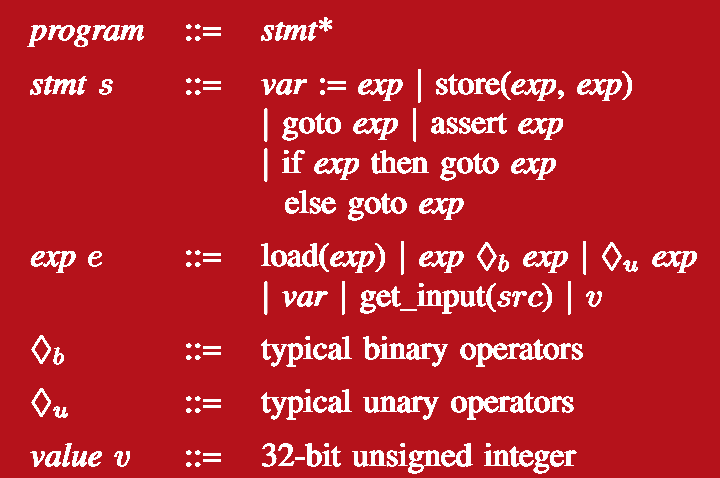
\includegraphics[scale=0.30]{SimpIL}
			\newline
			\textbf{SimpIL Grammar}
		\end{center}
	}
%	\only<2>{
%		\begin{itemize}
%			\item \textbf{Each} statement rule of the operational semantic is like:
%		\end{itemize}
%		\begin{prooftree}
%			\AxiomC{computation}
%			\UnaryInfC{$\textless$current state$\textgreater$, stmt $\rightarrow$ $\textless$end state$\textgreater$, stmt’}
%		\end{prooftree}
%		\begin{itemize}
%			\item The \texttt{state} is composed of: \newline
%		\begin{minipage}{0.5\textwidth}
%			\begin{itemize}
%				\item Program statements (\bm{$\sum$})
%				\item Current memory state (\bm{$\mu$})
%				\item Current values for variables (\bm{$\Delta$})
%			\end{itemize}
%		\end{minipage}
%		\begin{minipage}{0.4\textwidth}
%			\begin{itemize}
%				\item Program counter (\textbf{\textit{pc}})
%				\item Current statement (\textit{\textbf{i}})
%			\end{itemize}
%		\end{minipage}
%	\end{itemize}
%	}
\end{frame}
	
	
	
	%bibliography
	\newpage
	\nocite{*}
	\printbibliography % equivale a dare un \printbibliography per ogni categoria
	
\end{document}